% 2008 年山东卷文科第 3 题：函数 y=ln(cos x)（-π/2<x<π/2）图象的四个候选。
% 来源 PDF：gaokaomath-src/普通高考/2008/2008山东文.pdf
% SHA-256：479a9abc0fe5954c5b717d8eb0f649966c1cee3cfabdab00f10cc5834668fd6f
% 原页：2008山东文.pdf 第 1 页（A3 三栏）第 1 栏，书页码 473。
% 布局：四幅小图按 2×2 排布（行距 5.6 单位、列距 4.3 单位），每幅含 x、y 轴、
%   ±π/2 两条虚线渐近线与曲线，(A)～(D) 标在各小图正下方。
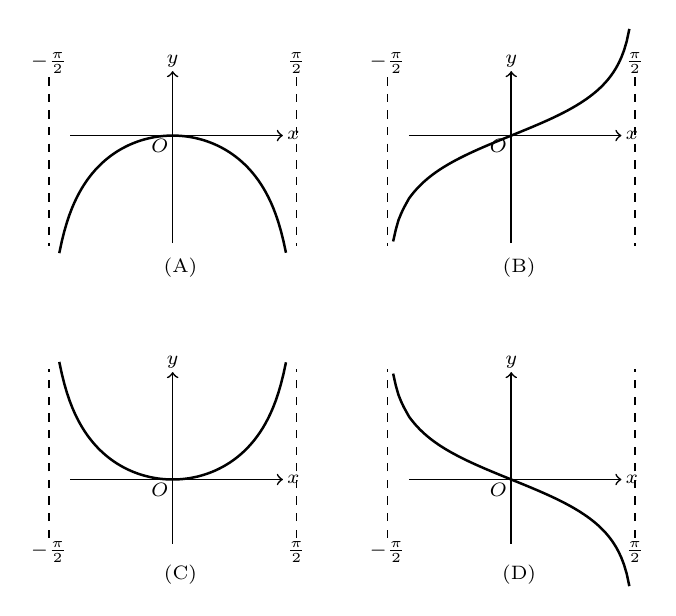
\begin{tikzpicture}[x=1.0cm, y=0.78cm, semithick, font=\scriptsize,
  every node/.style={inner sep=1.2pt}]

  % ---- (A) y = ln(cos x)：偶函数，x=0 处取最大值 0，两端趋于 -inf ----
  \begin{scope}[shift={(0,0)}]
    \draw[->] (-1.30,0) -- (1.40,0) node[right] {$x$};
    \draw[->] (0,-1.75) -- (0,1.05) node[above] {$y$};
    \node[below left] at (0,0) {$O$};
    \draw[dashed] (-1.571,0.95) -- (-1.571,-1.80);
    \draw[dashed] (1.571,0.95) -- (1.571,-1.80);
    \node[above] at (-1.571,0.95) {$-\frac{\pi}{2}$};
    \node[above] at (1.571,0.95) {$\frac{\pi}{2}$};
    \draw[line width=0.9pt, domain=-1.44:1.44, samples=90] plot (\x, {0.95*ln(cos(\x r))});
    \node at (0.10,-2.15) {(A)};
  \end{scope}

  % ---- (B) 递增且过原点 ----
  \begin{scope}[shift={(4.3,0)}]
    \draw[->] (-1.30,0) -- (1.40,0) node[right] {$x$};
    \draw[->] (0,-1.75) -- (0,1.05) node[above] {$y$};
    \node[below left] at (0,0) {$O$};
    \draw[dashed] (-1.571,0.95) -- (-1.571,-1.80);
    \draw[dashed] (1.571,0.95) -- (1.571,-1.80);
    \node[above] at (-1.571,0.95) {$-\frac{\pi}{2}$};
    \node[above] at (1.571,0.95) {$\frac{\pi}{2}$};
    \draw[line width=0.9pt, domain=-1.50:1.50, samples=90]
      plot (\x, {0.52*ln((1+sin(\x r))/cos(\x r))});
    \node at (0.10,-2.15) {(B)};
  \end{scope}

  % ---- (C) y = -ln(cos x) ----
  \begin{scope}[shift={(0,-5.6)}]
    \draw[->] (-1.30,0) -- (1.40,0) node[right] {$x$};
    \draw[->] (0,-1.05) -- (0,1.75) node[above] {$y$};
    \node[below left] at (0,0) {$O$};
    \draw[dashed] (-1.571,-0.95) -- (-1.571,1.80);
    \draw[dashed] (1.571,-0.95) -- (1.571,1.80);
    \node[below] at (-1.571,-0.95) {$-\frac{\pi}{2}$};
    \node[below] at (1.571,-0.95) {$\frac{\pi}{2}$};
    \draw[line width=0.9pt, domain=-1.44:1.44, samples=90] plot (\x, {-0.95*ln(cos(\x r))});
    \node at (0.10,-1.55) {(C)};
  \end{scope}

  % ---- (D) 递减且过原点 ----
  \begin{scope}[shift={(4.3,-5.6)}]
    \draw[->] (-1.30,0) -- (1.40,0) node[right] {$x$};
    \draw[->] (0,-1.05) -- (0,1.75) node[above] {$y$};
    \node[below left] at (0,0) {$O$};
    \draw[dashed] (-1.571,-0.95) -- (-1.571,1.80);
    \draw[dashed] (1.571,-0.95) -- (1.571,1.80);
    \node[below] at (-1.571,-0.95) {$-\frac{\pi}{2}$};
    \node[below] at (1.571,-0.95) {$\frac{\pi}{2}$};
    \draw[line width=0.9pt, domain=-1.50:1.50, samples=90]
      plot (\x, {-0.52*ln((1+sin(\x r))/cos(\x r))});
    \node at (0.10,-1.55) {(D)};
  \end{scope}
\end{tikzpicture}
